% ch2p13_001: Filling and drawing
\documentclass[tikz, border=10pt]{standalone}

\usepackage{tikz}

\begin{document}
	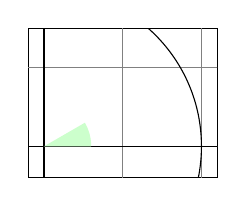
\begin{tikzpicture}[scale=2]
		\clip[draw] (-0.1, -0.2) rectangle (1.1, 0.75);
		
		\draw[step=0.5cm, gray, very thin] (-1.4, -1.4) grid (1.4, 1.4);
		\draw (-1.5, 0) -- (1.5, 0); % x-axis
		\draw (0, -1.5) -- (0, 1.5); % y-axis
		\draw (0, 0) circle [radius=1cm];
		
		% green 20% and white 80%
		% And the last `(0, 0)` was to close the path
		% \fill[green!20!white] (0, 0) -- (3mm, 0mm)
		% 	arc [start angle=0, end angle=30, radius=3mm] -- (0, 0);
			
		% Better option to close the path is to use `cycle`.
		\fill[green!20!white] (0, 0) -- (3mm, 0mm)
		arc [start angle=0, end angle=30, radius=3mm] -- cycle;
	\end{tikzpicture}
\end{document}